% Reflexion der eigenen Arbeit, ungelöste Probleme, weitere Ideen.

\chapter{Ausblick}\label{ausblick}
In diesem Kapitel werden möglich nächste Schritte für die Weiterentwicklung des DlmsQuickAccess aufgelistet.
Diese basieren auf  Rückmeldungen von Nutzern, Erkenntnissen aus dem Entwicklungsprozess oder auf geplanten Features welche in den sechs Sprints nicht umgesetzt werden konnten.  
Diese Arbeiten wurden in \ac{ADO} als User Story oder Bug erfasst, so dass sie von der Landis+Gyr priorisiert und eingeplant werden können.
Ein Ausschnitt aus diesem Backlog ist in Abbildung \ref{fig:ADOBacklog} gezeigt.
Ebenfalls reflektiert der Autor der Autor der Arbeit das Projekt.
\begin{figure}[H]
   \centering
   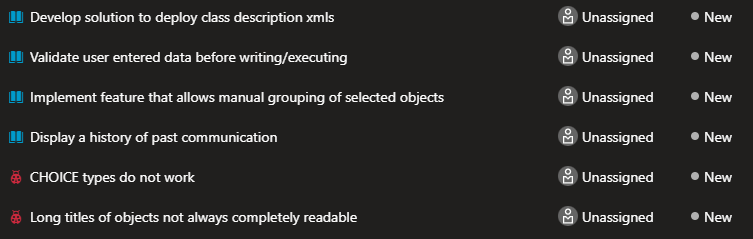
\includegraphics[width=1.0\textwidth]{gfx/ADOBacklog.png}
   \caption{
      Ausschnitt aus dem Backlog in \ac{ADO}
      }
   \label{fig:ADOBacklog}
\end{figure}


\section{Nächste Schritte}\label{nextSteps}
In den folgenden Abschnitten werden mögliche nächste Schritte aufgelistet.
Die Reihenfolge entspricht nicht einer Priorisierung sonder ist zufällig.

\subsection{Class Descriptions}
Die Class Descriptions, welche verwendet werden, um zusätzliche Informationen zu dem \ac{COSEM}-Objekten des Object Models darzustellen, sind Teil der Anwendung und werden bei der Installation auf den Rechner des Nutzers kopiert.
Um Änderungen an den Class Descriptions an die Nutzer zu verteilen muss jeweils eine neue Version der Anwendung veröffentlicht werden.
Da dies während dieses Projektes regelmässig gemacht wurde, waren die Class Descriptions bisher immer aktuell.
In der Zukunft sollte jedoch eine Lösung gefunden werden, bei welcher die Class Descriptions unabhängig von der Anwendung aktualisiert werden können.

\subsection{Eingabevalidierung}
-> ref auf Usability

\subsection{File Picker}\label{ausblick:filePicker}
Wird die Anwendung beim ersten Start ohne Konfigurationsdatei ausgeführt, so ist es für den Nutzer nicht möglich den DlmsQuickAccess richtig verwenden zu können.
Das Fenster, welches in Abbildung \ref{fig:welcomeScreenEmpty} gezeigt ist, weist ihn darauf hin, dass er die Anwendung über Eine *.dlmsquickaccess starten soll.
Es sollte jedoch auch möglich sein, eine Konfigurationsdatei mittels File Picker auswählen zu können.
In Abschnitt \ref{s3configvorgehen} ist beschrieben, wieso dies noch nicht umgesetzt werden konnte.

\begin{figure}[H]
   \centering
   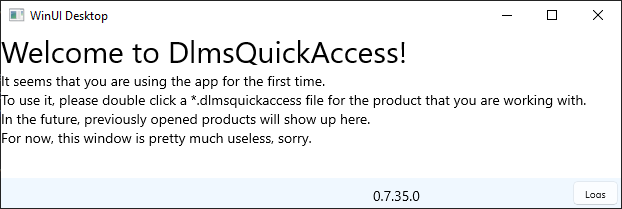
\includegraphics[width=1.0\textwidth]{gfx/welcomeScreenEmpty.png}
   \caption{
       Fenster des DlmsQuickAccess, welches erscheint, wenn die Anwendung ohne Konfiguration gestartet wird.
   }
   \label{fig:welcomeScreenEmpty}
\end{figure}

\subsection{Continuous Deployment}
TODO

\subsection{\ac{DMT2} Quick Access ablösen}
Wie im Abschnitt \ref{survey} beschrieben, wurden für diese Arbeit bewusst nur Entwickler aus Cham in den Entwicklungsprozess mit einbezogen.
Diese verwenden den DlmsQuickAccess in Kombination mit den Referenzprodukten der Picasso Platform.
Um die alte Software vollständig abzulösen, müssen Konfigurationen für weiter Produkte bereitgestellt werden sowie alle Entwickler mit dem DlmsQuickAccess bekannt gemacht werden.


\subsection{Sourcecode Organisieren}\label{ausblick:ats_split}
In diesem Projekt wurden Code von anderen C\# Anwendungen der Landis+Gyr verwendet.
Dazu wurden die Repositories dieser Anwendungen in das Repository des DlmsQuickAccess kopiert.
Wie das umgesetzt wurde ist im Abschnitt \ref{gitsubtree} aufgeführt.
Ein möglicher nächster Schritt wäre es, diese Abhängigkeiten neu zu organisieren.
Dazu müssten jene Teile des Codes, welche von DlmsQuickAccess benötigt werden, als NuGet Paket bereitgestellt werden.


\subsection{Testagent mit Zähler}
Im Abschnitt \ref{Integrationstests} wurde beschrieben, dass für das Ausführen der Integrationstests ein angeschlossener Stromzähler benötigt wird.
Beim Testagent, welcher die Tests in \ac{ADO} ausführt, ist kein solcher Zähler vorhanden.
Deshalb konnten die Integrationstest nur lokal ausgeführt werden.
Um in Zukunft sicherstellen zu können, dass neue Änderungen keine bestehenden Funktionen zerstören, wäre es ein möglicher nächster Schritt, einen Testagent mit angeschlossenem Stromzähler aufzusetzen.

\subsection{SonarQube}
In Abschnitt \ref{s6:sonar} wurde erklärt, wieso im Rahmen dieser Arbeit lediglich eine lokale Instanz des Qualitätssicherungstools SonarQube eingesetzt wurde.
Für den Unterhalt und die Weiterentwicklung der Anwendung sollte jedoch eine Instanz auf einem Server eingesetzt werden, welche mit dem \ac{CI} Server verbunden ist.
Dies hätte zwei Vorteile:
\begin{itemize}
   \item Die Berichte zu Codequalität werden bei jeder Änderung des Codes automatisch erstellt. 
Entwickler müssen sich nicht selber darum kümmern.
   \item Die Metriken zur Qualität der Anwendung sind für alle Personen einsehbar.
\end{itemize}


\subsection{Zertifikat für die Signierung der Anwendung}\label{ausblick:cert}
Im Abschnitt \ref{deployment} wurde erklärt, wie das Deployment der Anwendung umgesetzt wurde.
Dabei wurde die Schwierigkeit beschrieben, dass jeder Nutzer der Anwendung manuell ein Zertifikat einrichten muss, um die Anwendung installieren zu können.
Dieses Zertifikat gibt den Autor dieser Arbeit und nicht die Landis+Gyr als Ersteller der Anwendung an.
Das Zertifikat könnte durch eines der Landis+Gyr ersetzt werden, welches auf den Rechnern der Nutzer bereits vorhanden ist.


\subsection{History}
Vergangene Kommunikationen und deren Resultate sollen gespeichert und für die Nutzer dargestellt werden.
Bei Schreibbefehlen sollen die verwendeten Parameter angezeigt werden.
Eine Funktion, einen Befehl aus der History mit den selben Parametern zu wiederholen wäre ebenfalls erdenklichen.
Bereits bei der Umfrage \ref{survey} zu Beginn des Projekts wurde dieses Feature von den Nutzer hoch priorisiert.

\subsection{Gruppen}
Es soll für die Nutzer möglich sein, Gruppen von Objekten oder Attributen rsp. Methoden zu erstellen.
Diese sollen ähnlich wie die Favoriten dargestellt werden.
Eine Gruppe sollte als beispielsweise \ac{YAML}-Datei exportiert und importiert werden können.
Diese könnte dann einem Bug oder einer User Story angehängt werden dem Bearbeiter dieser den Zugriff auf relevante Objekte erleichtern.

\subsection{Exportieren von Daten}
Es soll möglich sein, gelesene Daten zu exportieren.
In folgenden Fällen wäre dies hilfreich:
\begin{itemize}
   \item um ausgelesene Daten zu vergleichen
   \item um die Daten einer User Story oder einem Bug anzufügen
   \item für die Weiterverarbeitung der Daten
\end{itemize}

\subsection{Tastenkombinationen}
Um die Usability der Anwendung zu erhöhen sollen Tastenkombinationen für das ausführen von Operation hinzugefügt werden.
Wie in Abschnitt \ref{gefundeneFehler} aufgeführt, wurde von den Nutzern gewünscht, dass die Suche über eine Tastenkombination ausgeführt werden kan.
Das Lesen und das Schreiben von Attributen wären ebenfalls Kandidaten für Tastenkombinationen.







\section{Reflexion}